
% This template has been edited from the IEEE template available at:
% https://www.ieee.org/conferences/publishing/templates.html
%
% For further help, you may wish to see:#
% https://www.overleaf.com/learn/latex/tables
% https://www.overleaf.com/learn/latex/Inserting_Images
% https://www.overleaf.com/blog/532-creating-and-managing-bibliographies-with-bibtex-on-overleaf

\documentclass[conference]{IEEEtran}
%\IEEEoverridecommandlockouts
% The preceding line is only needed to identify funding in the first footnote. If that is unneeded, please comment it out.
\usepackage{cite}
\usepackage{amsmath,amssymb,amsfonts}
\usepackage{algorithmic}
\usepackage{graphicx}
\usepackage{textcomp}
\usepackage{xcolor}
\usepackage{subfigure}
\usepackage{parskip}
\usepackage{stfloats}
\usepackage{algorithm}
\usepackage{algpseudocode}
\usepackage{amsmath}
\renewcommand{\algorithmicrequire}{\textbf{Input:}} % Use Input in the format of Algorithm
\renewcommand{\algorithmicensure}{\textbf{Output:}} % Use Output in the format of Algorithm

\def\BibTeX{{\rm B\kern-.05em{\sc i\kern-.025em b}\kern-.08em
  T\kern-.1667em\lower.7ex\hbox{E}\kern-.125emX}}
\begin{document}

\title{Comparing Two Different Complete Coverage Path Planning Algorithms Using The E-puck In Webots}

\author{
  \IEEEauthorblockN{Daoming Chen}
  \textit{Department of Engineering Mathematics}\\
  \textit{University of Bristol,UK}
  \IEEEauthorblockN{ta21463@bristol.ac.uk}
  \and
  \IEEEauthorblockN{Yifan Wang}
  \textit{Department of Engineering Mathematics}\\
  \textit{University of Bristol,UK}
  \IEEEauthorblockN{rj21561@bristol.ac.uk}
}

\maketitle

\begin{abstract}
The path planning algorithm is the basis for selecting the optimal route between two points in a map environment for a mobile robot. Among path planning algorithms, the complete coverage path planning algorithm is a method that allows a mobile robot to traverse every point in a map, given a known map environment. This method determines how efficiently the robot vacuum cleaner can complete its tasks. The two main complete path planning algorithms on the market for robot vacuum cleaners are the Boustrophedon Cell Decomposition and the Backtracking Spiral Algorithm. This paper simulates and tests the E-punk autonomous mobile robot in different map environments using two algorithms on the Webots simulation platform. This paper also conducts experiments comparing the completion efficiency of the two algorithms in different map environments. The experimental results positively reference to the robot vacuum cleaner development team.
\end{abstract}

\def\IEEEkeywordsname{Keywords} 
\begin{IEEEkeywords} Coverage  Path  Planning, Webots simulation, Efficiency comparison experiments 
\end{IEEEkeywords} 

\section{Introduction}
With the development of mobile robotics and the continuous innovation of robot vacuum cleaner products, path planning algorithms have become particularly important. Path planning algorithms aim to find an optimal path for a mobile robot, which at the same time satisfies that the path always does not intersect any obstacle from the starting point to the ending point in a given environment. The path trajectory generated by the robot path planning plays a navigational role in its movement and guides the robot from the current point to the target point avoiding obstacles. Complete coverage path planning(CPP) is the process of determining the feasible or optimal path trajectory by delineating the boundaries of obstacle and free areas and ensuring that all points in a given environment are visited at least once, given that all spatial maps information is known. CPP algorithm is widely used in robot vacuum cleaners\cite{colegrave1994case}.\\
The Boustrophedon Cell Decomposition (BCD)\cite{lavalle2006planning} and the Backtracking Spiral Algorithm (BSA)\cite{gonzalez2005bsa} are two CPP methods. These two methods are the main methods used by robot vacuum cleaners. One of the reasons why the time to complete a task varies from one robot vacuum cleaner to another is the different choices of CPP algorithms. This work looks to compare the completion times of mobile robots returning to the starting point from the starting point using these two CPP algorithms in different environments to obtain a more efficient algorithm.

\section{Hypothesis Statement}
In the BCD algorithm, boustrophedon\cite{choset1998coverage} means the way ox walks which is the parallel line-covered areas. So the method traverses the entire map environment in parallel lines(see Fig.\ref{bcd}). While the BSA algorithm\cite{Gonzlez2003BSAAC} is filling rectangular regions using a spiral pattern(see Fig.\ref{bsa}).\\

\begin{figure}[htbp]
\centering
\begin{minipage}[t]{0.48\textwidth}
\centering
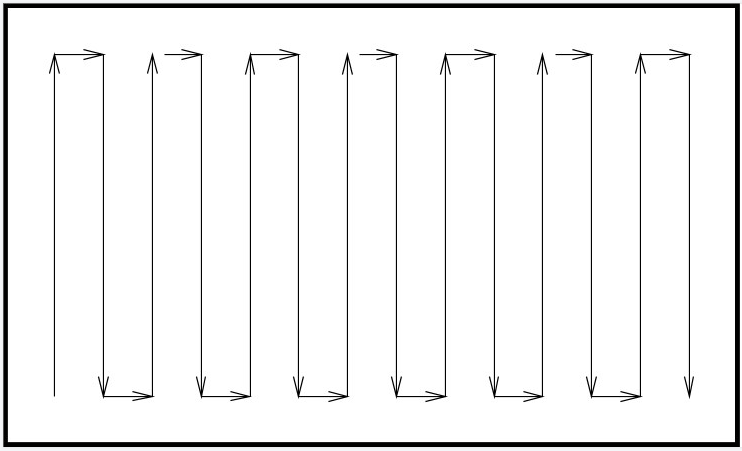
\includegraphics[width=6cm,height=4cm]{RS_Report/bcd.png}
\caption{Diagram of the BCD algorithm\cite{choset1998coverage}. }
\label{bcd}
\end{minipage}
\begin{minipage}[t]{0.48\textwidth}
\centering
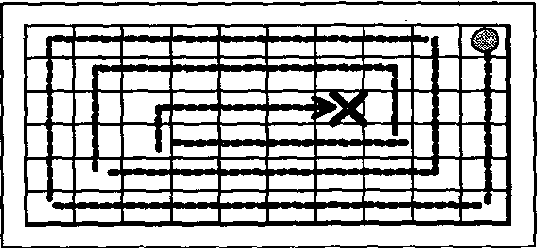
\includegraphics[width=6cm,height=4cm]{RS_Report/BSA.png}
\caption{Diagram of the BSA algorithm\cite{Gonzlez2003BSAAC}.}
\label{bsa}
\end{minipage}
\end{figure}

There is a clear difference between the two algorithms. The BCD algorithm has a tighter overall path because of its 180° turns, which are closer together after each turn, In the BSA algorithm, because of its 90° turns after encountering an obstacle, which is not close together after the turn. BSA algorithm is an outward-to-inward spiral path planning method, and its external route will create a certain distance from the internal route. Its route continuity caused by turning when random obstacles appear in the environment will be relatively poor compared to the BCD algorithm.
Based on these observations, a hypothesis has been developed stating:
\begin{quote}
   In a blank map environment, BCD is similarly efficient to BSA because there are no extra routes in the path due to the A* algorithm. However, in the complex map environment (containing random obstacles), with the addition of the A* routes, BCD with compact paths is more efficient than BSA.
\end{quote}

\section{Implementation}
The individual functions and algorithms required during the experiments were tested separately and a map environment (with obstacles) was built for the experiments.


\subsection{Map and track tracking system}

The premise of the complete coverage path plan algorithm is a map and locate system. Only when the robot knows the surrounding environment and its position can it make a reasonable path plan.

\subsubsection{Map}

There are various methods to build the environment map, and this experiment mainly uses the raster method\cite{hart1968formal} to build the environment map in a static environment.This method is used because it decomposes the environmental space in to local cells and describes the state of the environment in terms of whether obstacles occupy them or not. The maps produced by this method provide accurate metric information and are easier to understand and process than other methods. Algorithms are compared in 90cm×90cm rectangular maps(see Fig.\ref{fig1}) with obstacles. The robot will receive a static 11×11 raster map (see Fig.\ref{fig2}) at the beginning of the experiment. On the map, cells that contains obstacles or wall are set to 1, and cells that the robot can step on are set to 0.

\begin{figure}[htbp]
\centerline{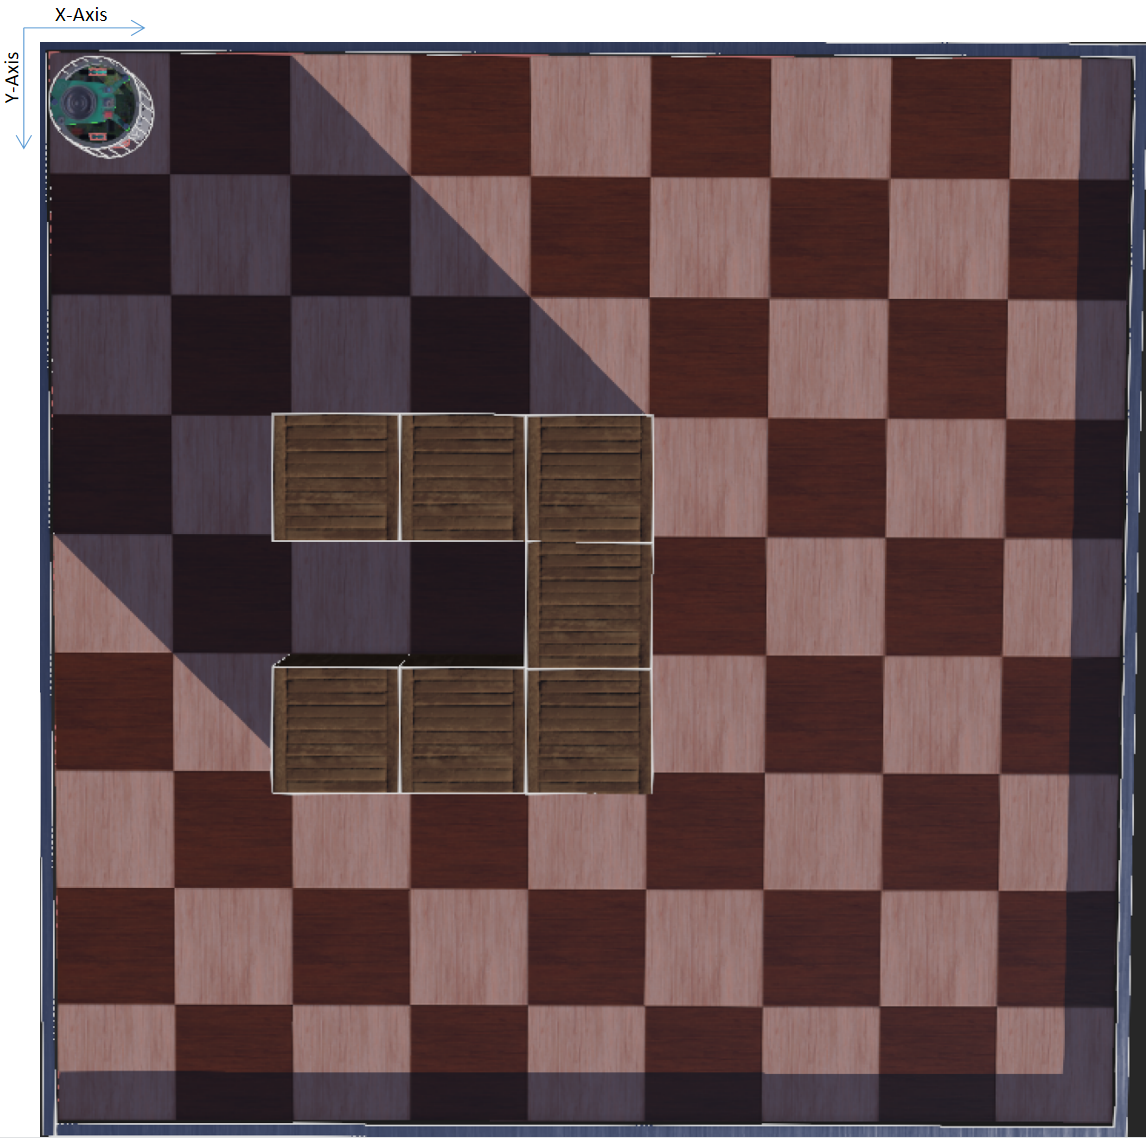
\includegraphics[width=5cm,height=5cm]{RS_Report/Webots_map.png}}
\caption{E-punk campaign map built in Webots.}
\label{fig1}
\end{figure}

\begin{figure}[htbp]
\setlength{\belowcaptionskip}{-1cm}
\centerline{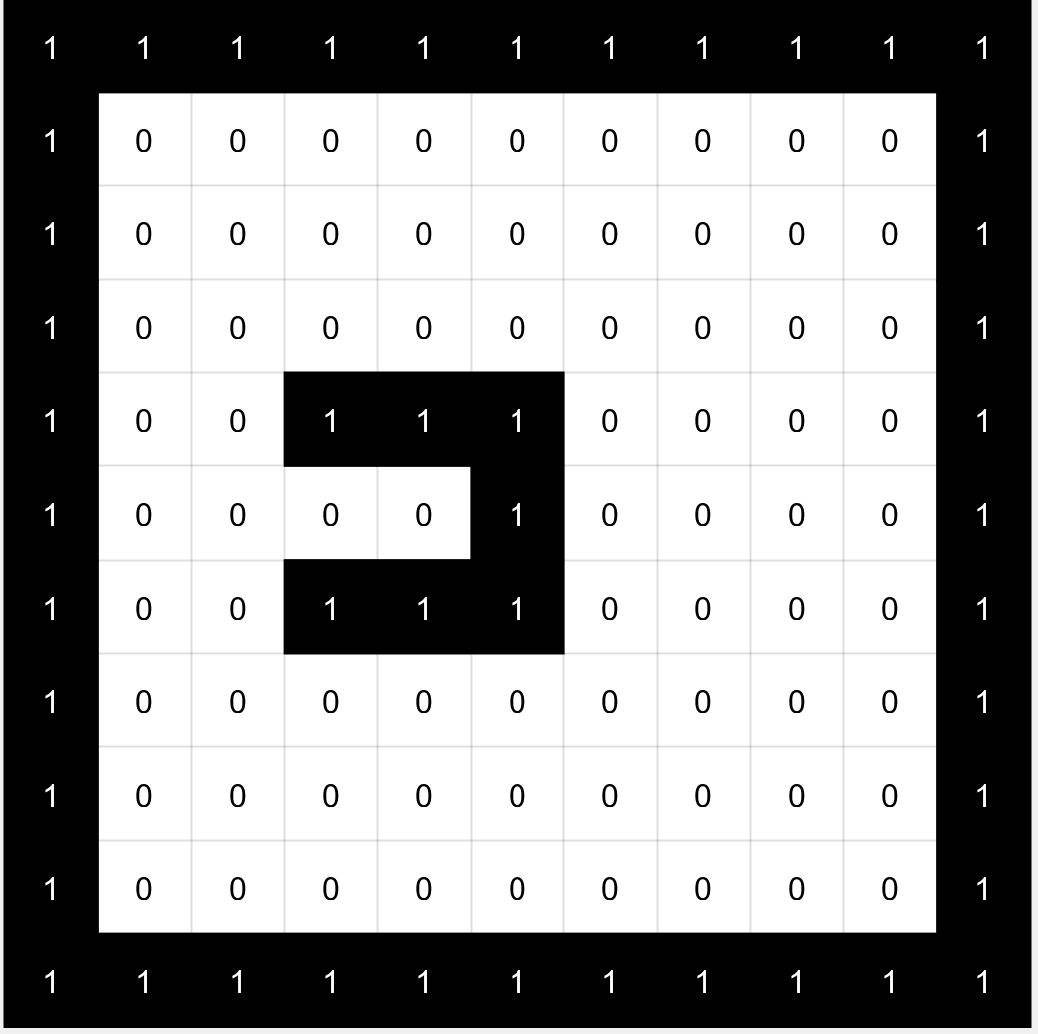
\includegraphics[width=5cm,height=5cm]{map.png}}
\caption{Raster environment map built for E-punk.}
\label{fig2}
\end{figure}

\subsubsection{E-punk pose}

In order to obtain the pose of the robot, the supervisor system of Webots is enabled in this experiment. The supervisor system can obtain the absolute position and orientation of the robot in the simulator. The position is information is a three by one translation vector from the simulator's origin to the robot. In this experiment, only x and y are used. The orientation information is returned as Euler angle from the simulator's origin to the robot. Since the robot only walk on the plane perpendicular to the y axis in this experiment, the only useful parameters are the direction of y axis and its angle. The pose of the robot on the map can be obtained by converting the pose obtained from the supervisor. 

\subsubsection{Track tracking}

By storing the pose data of the robot in a list in order, we can get the robot's motion trajectory. In order to more intuitively understand which areas on the map are covered, this trajectory needs to be marked on the map. The 11×11 raster map can only display the position of the robot in integer. Therefore, each punctuation is made when the robot is at the center of the grid. On the raster map, when a cell is covered, the value will change from 0 to 2.

\subsection{CPP algorithm}

Fig.\ref{fig3} shows the overall form of the algorithm architecture combining the map, A* algorithm and CPP algorithm. The architecture allows E-punk to complete the map traversal and compare the completion times of the two different CPP algorithms. 

\begin{figure}[htbp]
\setlength{\belowcaptionskip}{-1cm}
\centerline{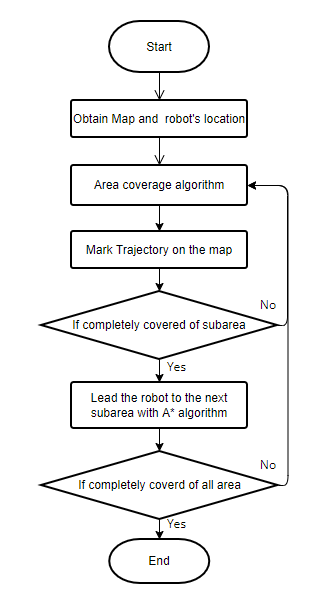
\includegraphics[scale=0.8]{RS_Report/The Overall architecture of the CPP algorithm.png}}
\caption{The Overall architecture of the CPP algorithm.}
\label{fig3}
\end{figure}
 
\subsubsection{A* algorithm}
The sweeping robot returns to the initial point to recharge after completing the cleaning task in the real world. In this experiment, the robot is set to return to its initial position after completing the CPP task, which is designed to simulate the realistic motion of the robot better. The A* algorithm\cite{hart1968formal} is used to return to the initial position more quickly and with the shortest path.\\
As E-punk traverses the map, there will always be places that it has not traversed in a single loop. In this case, the experiment uses the A* algorithm to move the cart to the nearest untraversed region until the entire map is traversed.\\
The core of the a* algorithm is
\begin{equation}
  f(n) = g(n) + h(n)
\end{equation}
where $f(n)$ is the combined priority of node n. When the next node to be traversed needs to be selected, the algorithm always picks the node with the highest combined priority (smallest value). $g(n)$ is the cost of node n from the starting point. $h(n)$ is the expected cost of node n from the end point, which is the heuristic function of the A* algorithm.\\
The traversal direction is simplified in this experiment to match the raster map and speed up the calculation. The mobile robot can only move in four directions, up, down, left and right, in which case the heuristic function is calculated using the Manhattan distance method(see Fig.\ref{fig4}).

\setlength{\belowcaptionskip}{-1cm}
\begin{figure}[htbp]
\centerline{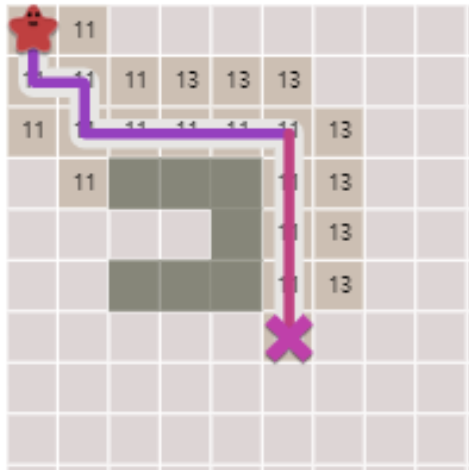
\includegraphics[width=5cm,height=5cm]{RS_Report/astar.png}}
\caption{A* algorithm demonstration(the value in the cell is the value of $f(n)$).}
\label{fig4}
\end{figure}

\subsubsection{Area coverage path plan algorithm}

The BCD and BSA area coverage algorithms(see Algorithm\ref{alg.l1}) are design with the same finite state machine, but with different motion rules. The robot will behave as the algorithm instructs in different scenarios. The scenarios based on the map and track tracking system updates at a rate of 31.25Hz. The main difference between BCD and BSA lies in the way they turn. The BCD will turn the robot 180 degree in U-shape. The BSA will let the robot implement a 90-degree round turn. 


\begin{algorithm}[h]
 \caption{Area coverage path plan algorithm}
 \label{alg.l1}
 \begin{algorithmic}[1]
 \Require
 Map; Robot's position on the map;
 \Ensure
 Robot's behavior;
 
    \STATE Wall = 1;
    \STATE Trajectory = 2;
    \STATE Blank = 0;
    \STATE $\textit{Position} \gets \text{Robot's current position on the map}$
    \STATE $\textit{Front} \gets \text{One cell in front of } \textit{Position}$
    \STATE $\textit{Left} \gets \text{The cell to the left of } \textit{Position}$
    \STATE $\textit{Right} \gets \text{The cell to the right of } \textit{Position}$
    {\IF{Front \textgreater 0}
        \IF{Left \textgreater 0}
            {\IF{Right \textgreater 0}
                {The area is fully covered}
            {\ELSE}
                {Turn right}
            \ENDIF
        {\ELSIF{Right \textgreater 0}
            {Turn right}}
        \ENDIF}
  \ENDIF}
  \label{code:recentEnd}
 \end{algorithmic}
\end{algorithm}

\section{Experiment Methodology}

\subsection{Overview of Method}
The experiments need to compare the efficiency performance of the two algorithms, BCD and BSA, in different map environments. The experiments first compared the performance of the two algorithms in a simple map environment (a blank map without obstacles).\\
After completing the experiment in the blank map, two complex maps (containing obstacles) were created and the performance of BCD and BSA was compared in the two complex maps. The overall layout of the room on the floor for the robot vacuum cleaner does not usually change significantly except for the movement of people, so in this experiment, all maps are static maps, and obstacles do not move. This section is the central part of the experiment. A 90mm$\times$90mm map was defined, and 10mm$\times$10mm square obstacles were placed at random locations on the map. After the map was constructed, the performance of the two path planning algorithms was compared. After comparing on this map environment, the experiment was carried out in another different map environment. This approach aims to reduce the impact of random errors in path planning caused by the particular location of some map obstacles. Because the Webots simulation software came with a time counter, the completion time was output when the simulation of both path algorithms ended. Webots is a simulator where the experiment does not require multiple experiments in a single environment to reduce random errors. During the E-punk's movement, the coordinates of the locations it travelled were recorded in real-time, and the set of path coordinates, which was used to visualise the route, was exported when the task was completed.
\subsection{Discussion of Variables}
In this experiment, it is necessary to control that the initial conditions are the same for both algorithms when comparing on the different complex maps. The starting position of the E-punk is the same for both algorithms. The experiments all started at the global coordinate system $(x, y, \theta) = (0, 0, 0)$, which in the simulated map was located in the top left corner of the map (see Fig.\ref{fig1}). The E-punk's straight ahead speed and turning speed are constant for both path planning algorithms, and these two values do not change from one map to another. The heuristic function used in the A* algorithm is based on the Manhattan distance, which does not change during the comparison. The motion parameters in this algorithm are also unchanged.

\subsection{Discussion of Metric(s)}
As proposed in the hypothesis, the metric obtained was collected to evaluate the two path planning algorithms' efficiency and compare them. \\
Table \uppercase\expandafter{\romannumeral1} details the metric chosen for this experiment.

\begin{table}[htbp]
\centering
\setlength{\abovecaptionskip}{0.cm}
\caption{Definition of metrics and their sources}
\label{Table1}
\begin{tabular}{c|l|c}
\hline
Metric                & \multicolumn{1}{c|}{Source of Metric} & Justification     \\ \hline
Time(s)               & Internal timer            & Length of mapping time \\ \hline
\end{tabular}
\end{table}

The metric in this experiment can be obtained directly from the timer within Webots. In this experiment, as a measure of efficiency, it is better to measure time rather than distance travelled, as distance travelled does not consider the time taken to make a turn very well. 

\begin{figure*}[ht]
\centering
\setlength{\abovecaptionskip}{0.cm}
\subfigure[BCD route in the first complex map.]{
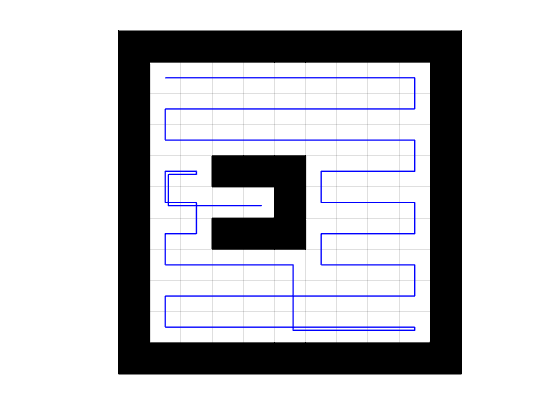
\includegraphics[width=8cm]{RS_Report/BCD_easy.png}
%\caption{fig1}
}
\quad
\subfigure[BSA route in the first complex map.]{
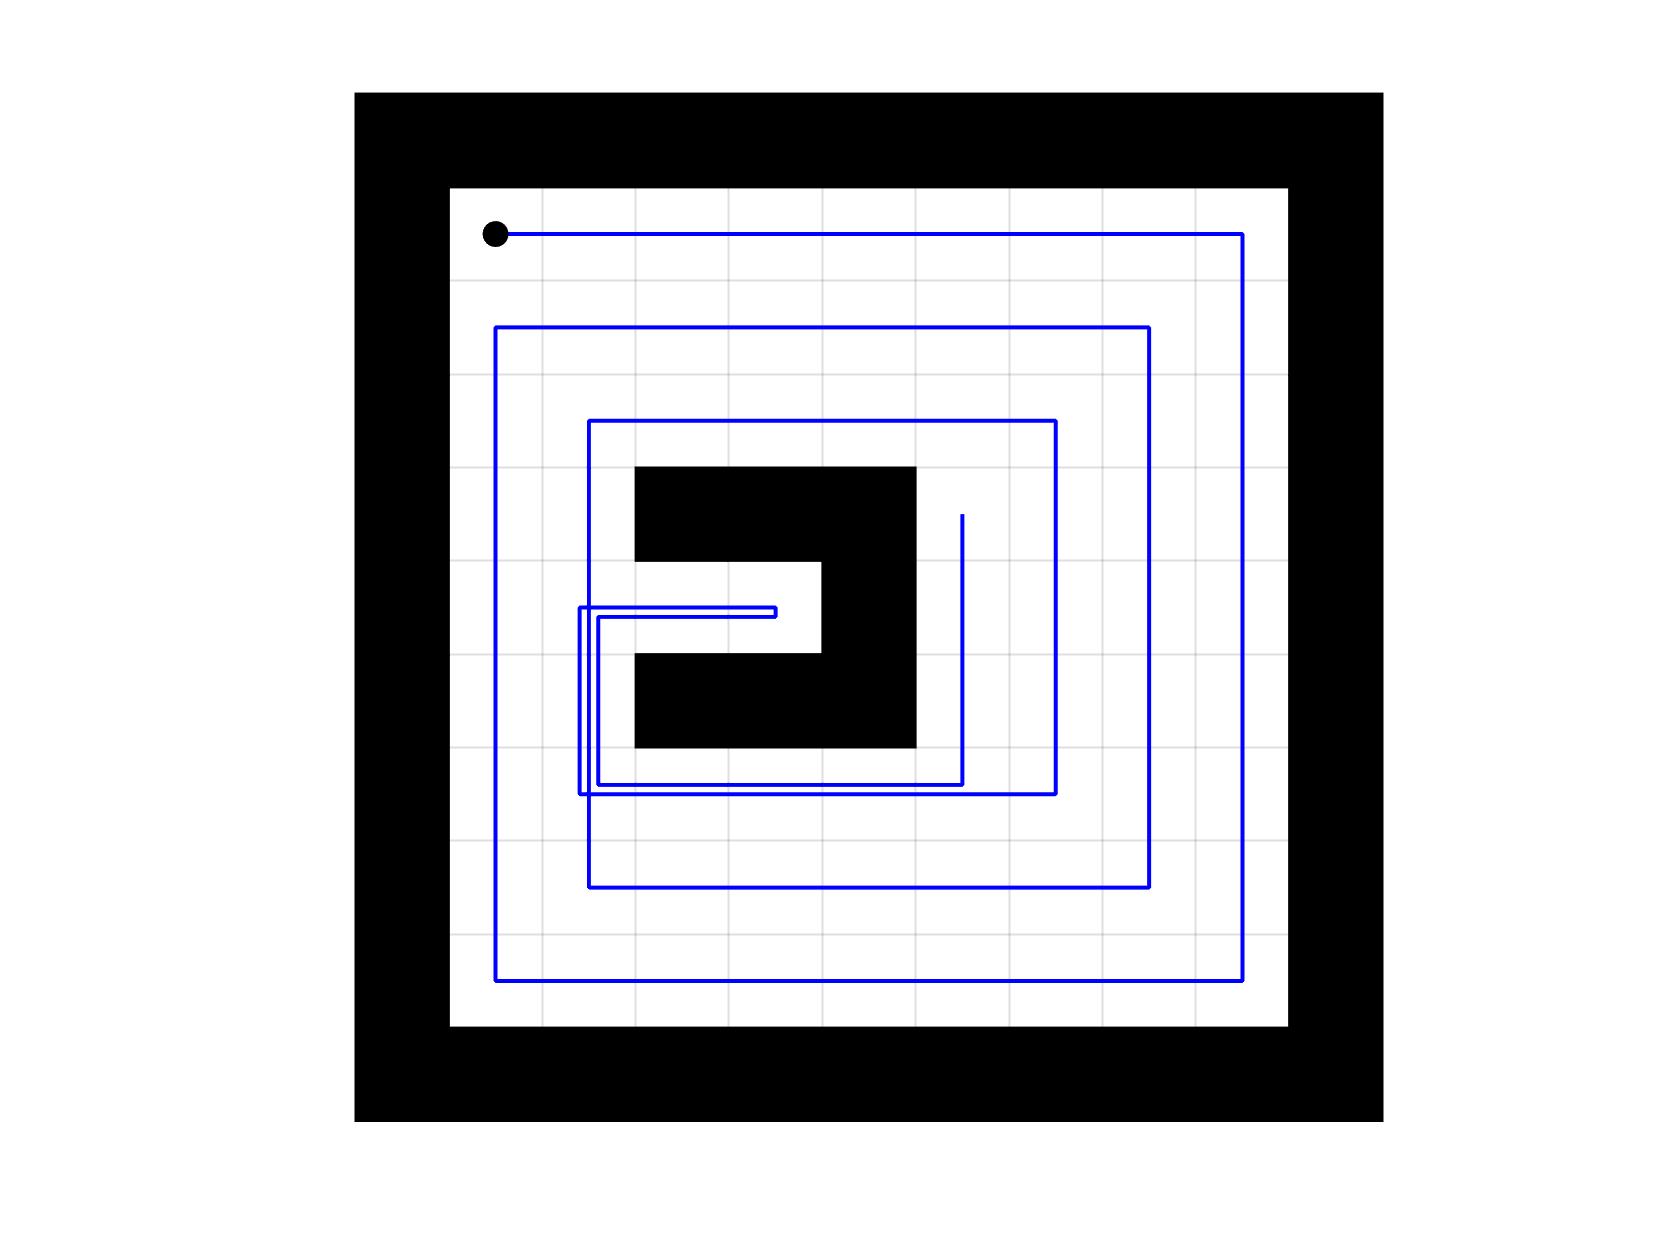
\includegraphics[width=8cm]{RS_Report/BSA_easy.png}
}
\quad
\subfigure[BCD route in the second complex map.]{
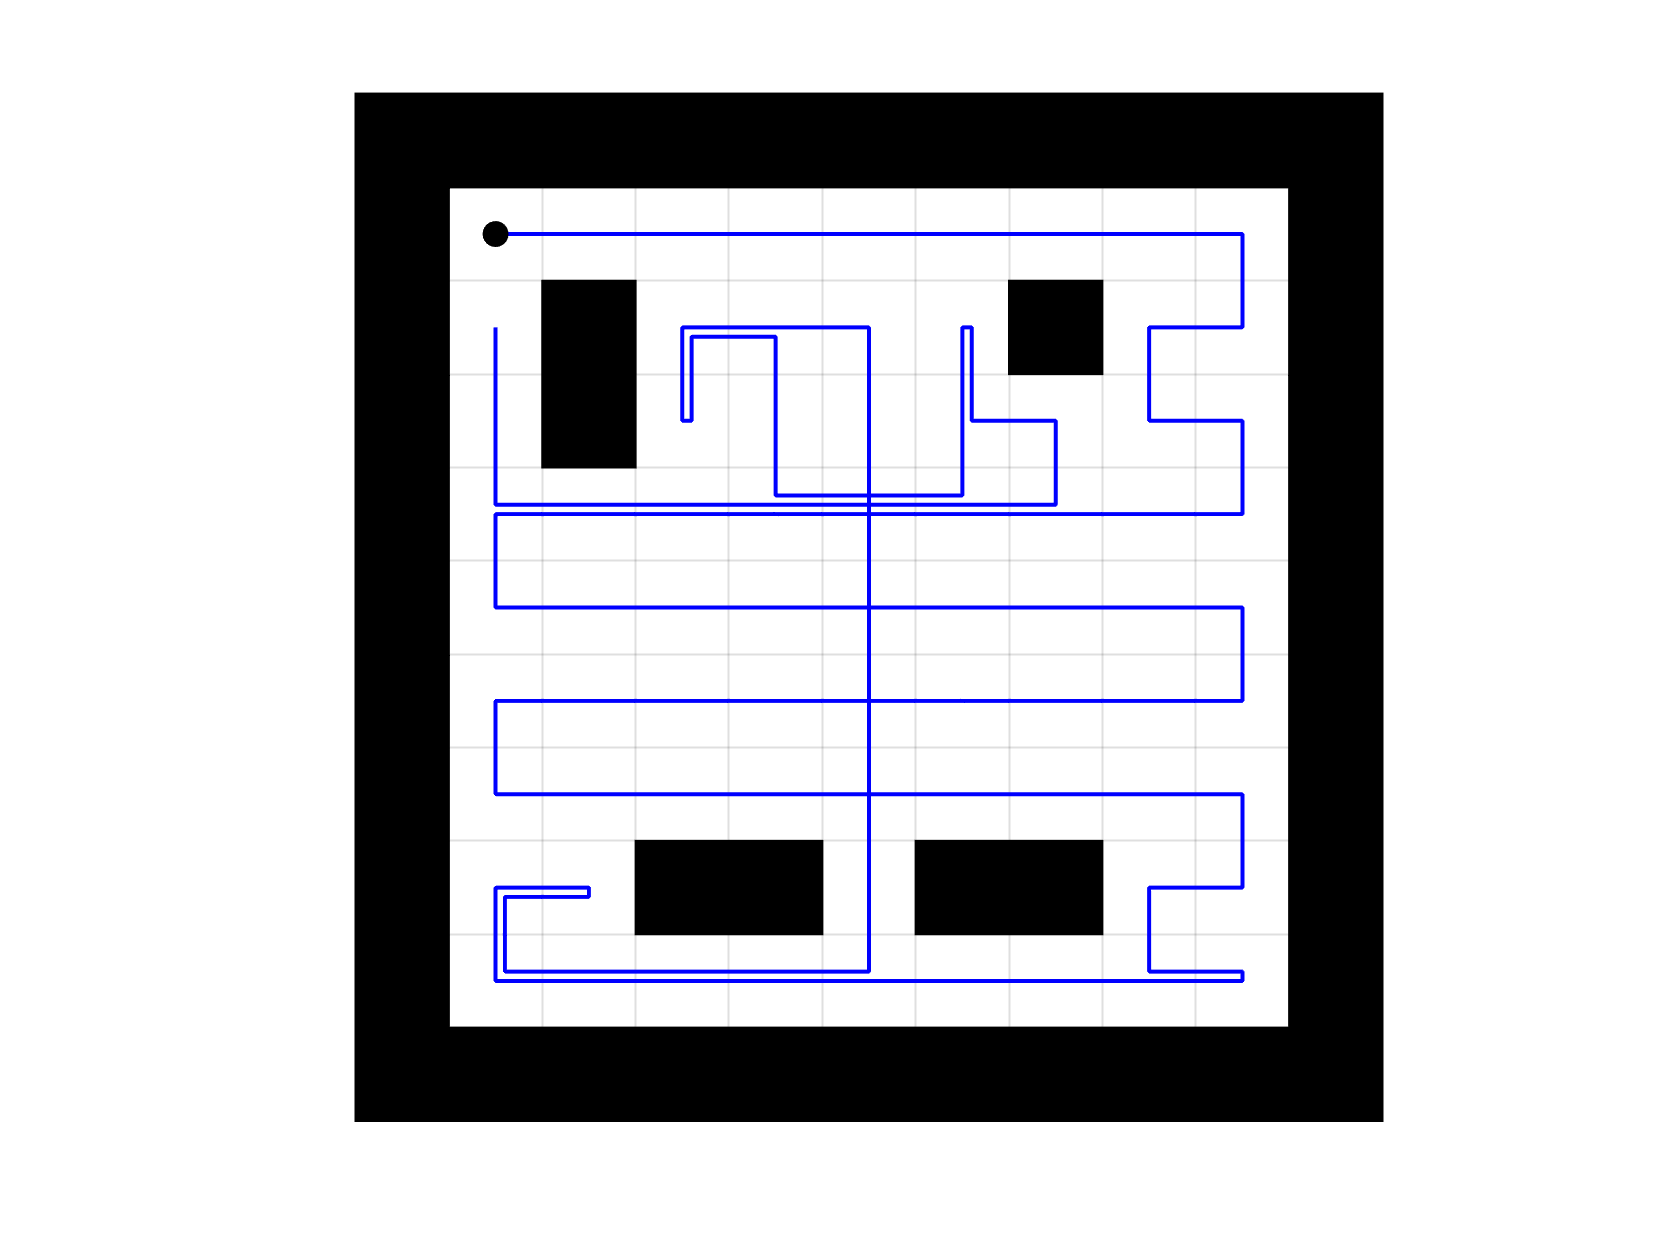
\includegraphics[width=8cm]{RS_Report/BCD_mid.png}
}
\quad
\subfigure[BSA route in the second complex map.]{
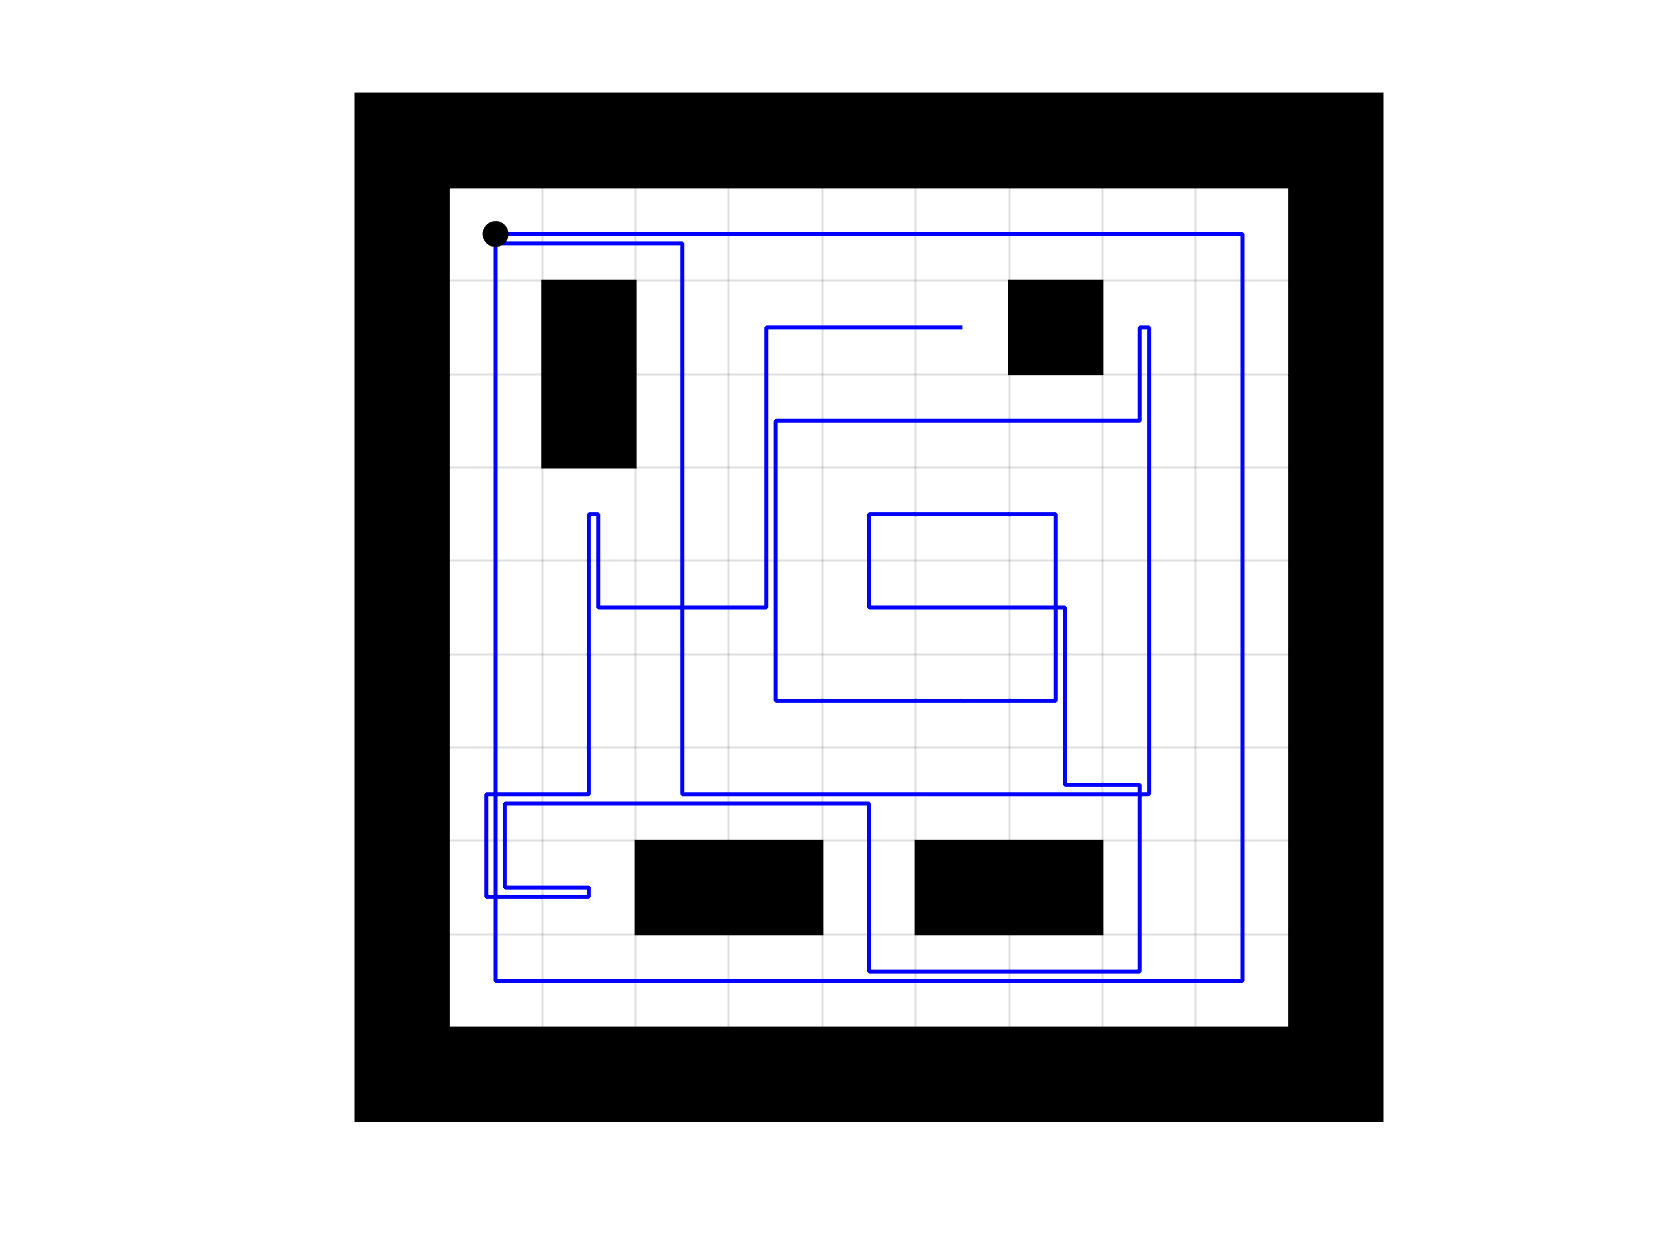
\includegraphics[width=8cm]{RS_Report/BSA_mid.png}
}
\caption{Path visualisation diagram for CPP algorithm}
\label{fig7}
\end{figure*}

% Please add the following required packages to your document preamble:
% \usepackage{graphicx}
\begin{table*}[bp]
\caption{Presentation of experimental results}
\label{Table2}
\resizebox{\textwidth}{!}{%
\begin{tabular}{ccccccc}
\hline
Map    & \multicolumn{2}{c}{Blank Map}               & \multicolumn{2}{c}{First Complex Map}           & \multicolumn{2}{c}{Second Complex Map} \\ \hline
Algorithm & \multicolumn{1}{c|}{BCD}  & \multicolumn{1}{c|}{BSA}  & \multicolumn{1}{c|}{BCD}  & \multicolumn{1}{c|}{BSA}  & \multicolumn{1}{c|}{BCD}   & BSA   \\
Time(s)  & \multicolumn{1}{c|}{225.57} & \multicolumn{1}{c|}{225.34} & \multicolumn{1}{c|}{315.90} & \multicolumn{1}{c|}{326.88} & \multicolumn{1}{c|}{401.76} & 412.70 \\ \hline
\end{tabular}%
}
\end{table*}


\section{Results and Analysis}
This experiment compares the BCD and BSA path planning algorithms in a blank map and two complex maps. The time at task completion was obtained using Webots internal timer, which was used to compare the efficiency of the two algorithms. The experimental results are shown in Table \uppercase\expandafter{\romannumeral2}. Fig.\ref{fig7} shows the trajectories of the different path planning algorithms in two complex maps.\\
In the blank map, BCD and BSA have similar completion times. The main reason for this result is that there is no significant difference between the lengths travelled by the two algorithms in this map. Furthermore, both algorithms have completed the map traversal without the help of the A* algorithm, and there is also no increase in distance travelled by the A* algorithm. So the efficiency of the two algorithms is similar in this case, which also verifies part of the experimental hypothesis.\\
Considering that a single map or particular obstacle placement may be advantageous for a specific algorithm, two different environments were compared in this experiment. In the first complex map environment, obstacles were concentrated in the middle of the map, while in the second complex map environment, obstacles were scattered around the map.\\
The experimental results show that BCD is more efficient in the first complex map. Both algorithms use the A* algorithm twice to help complete the map traversal, but it is clear that BSA is not as efficient as BCD because there is a longer A* path in the final path of BSA to complete the traversal. The map partitioning formed by BCD and BSA is different when path planning is completed. Because the route after a BCD turn is adjacent to the one before the turn, the area it passes through is also adjacent and does not result in a repeat of finding points in adjacent areas that have not been traversed. However, BSA does not achieve this effect, resulting in different partitions being far apart, and the efficiency is compromised if there are still obstacles in between.\\
In the second complex map, the BCD is still more efficient than the BSA compared to the results in the first complex map above, and the BCD is completed faster and more efficiently in this map.In the second complex map, the BSA algorithm still suffers from long partition distances and not close enough paths. It was also found that when the BSA algorithm encountered an obstacle, the BSA algorithm would miss the points around the obstacle, resulting in a less tight route. Moreover, during the whole map traversal process, the BSA needs to return to the previously traversed area and find the unreachable point several times with the A* algorithm, which will affect its efficiency.Compared to BSA, BCD is much more efficient at traversing the points around an obstacle, which is one reason why BCD is more efficient.From the path diagram of the second complex map, the experiments also revealed that because the BSA is a spiral inwards movement pattern, this tends to increase the distance of the spiral centroid from the next point found by the A* algorithm, thus increasing the time it takes to get to the next location.\\
In summary, BCD will be more efficient than BSA in complex environments. This is also in line with the experimental hypothesis. With this experiment, the accuracy of the experimental hypothesis was verified.

\section{Discussion and Conclusion}

Begin your discussion and conclusion by re-stating your hypothesis. You can literally copy-and-paste your hypothesis here. 

Because the VL1680X has been identified as an active sensor with ... limitations, we hypothesised that:
\begin{quote}
  by applying ... filtering to the sensor, we predict a measurable improvement of the sensor under ... conditions. 
\end{quote}


\bibliographystyle{ieeetr} 
\bibliography{biblio}


\end{document}
